\documentclass{beamer}
%
% Choose how your presentation looks.
%
% For more themes, color themes and font themes, see:
% http://deic.uab.es/~iblanes/beamer_gallery/index_by_theme.html
%
\mode<presentation>
{
  \usetheme{Warsaw}      % or try Darmstadt, Madrid, Warsaw, ...
  \usecolortheme{default} % or try albatross, beaver, crane, ...
  \usefonttheme{default}  % or try serif, structurebold, ...
  \setbeamertemplate{navigation symbols}{}
  \setbeamertemplate{caption}[numbered]
} 

\usepackage[english]{babel}
\usepackage[utf8x]{inputenc}

\title[]{Uma análise comparativa entre algoritmos estáticos para balanceamento de carga em redes SDN em ambiente IoT}
\author{Anselmo Battisti}
\institute{Universidade Federal Fluminense}
\date{Dezembro de 2018}

\begin{document}

\begin{frame}
  \titlepage
\end{frame}

% Uncomment these lines for an automatically generated outline.
%\begin{frame}{Outline}
%  \tableofcontents
%\end{frame}

\begin{frame}{Agenda}
    \begin{itemize}
      \item O Problema;
      \item Tecnologias e conceitos;
      \item Balanceamento estático de carga;
        \begin{itemize}  
            \item Random;
            \item Round Robin;
            \item Weighted Round Robin.
        \end{itemize} 
      \item O experimento;
      \item Resultados obtidos;
      \item Considerações finais.
    \end{itemize}
\end{frame}

\begin{frame}{O problema}

    \begin{block}
      
      Qual método utilizar para balancear de forma adequada os diversos fluxos existentes entre dispositivos IoT e os servidores de processamento em uma cidade inteligente que utilizada tecnologia SDN?
      
    \end{block}

    \vspace{0.2in}
    \textbf{Hipótese}
    \vspace{0.2in}
    
    \textit{h0: Não existe diferença significativa entre os tempo de resposta e a taxa de download entre os algorítimos de balanceamento de carga estáticos Random, Round Robin (RR) e Weighted Round Robin (WRR).}
\end{frame}

\begin{frame}{Tecnologias e conceitos}

    \begin{itemize}
      \item Cidades Inteligentes;
      \item Internet das Coisas;
      \item SDN.
    \end{itemize}

\end{frame}


\begin{frame}{Balanceamento estático de carga}

    \begin{block}{Balanceamento de Carga}
        Podemos dividir os algorítimos de balanceamento de carga em dois grupos: os \textbf{estáticos} e os \textbf{dinâmicos}.
    \end{block}

    Os algoritmos estáticos comparados nesse trabalho foram:
    
    \begin{itemize}  
        \item Random;
        \item Round Robin;
        \item Weighted Round Robin.
    \end{itemize}
\end{frame}
  
\begin{frame}{O Experimento}
    \begin{figure}[ht]
    \centering
    \includegraphics[width=0.6\textwidth]{images/network.png}
    \caption{Estrutura da rede utilizada para a realização dos testes}
    \label{fig:rede_proposta}
    \end{figure}
\end{frame}  
  
\begin{frame}{O Experimento}
    \begin{table}[]
    \centering
    \caption{Largura de banda de cada servidor em cada um dos experimentos, valores em MBits/seg}
    \label{largura_banda}
    \begin{tabular}{llllll}
     & H1 & H2 & H3  & H4 & H5 \\\hline
    Experimento 1                  & 1  & 2  & 4   & 8  & 16 \\
    Experimento 2                  & 10 & 10 & 10  & 10 & 10 \\
    Experimento 3                  & 5  & 5  & 7.5 & 10 & 10
    \end{tabular}
    \end{table}
\end{frame}    
  
\begin{frame}{Resultados obtidos - Experimento 1}

    Simula um cenário onde a larguras de banda definidas entre os servidores e o \textit{load balancer} tem uma variação exponencial.

    \begin{figure}[ht]
        \begin{minipage}[b]{0.45\linewidth}
            \centering
            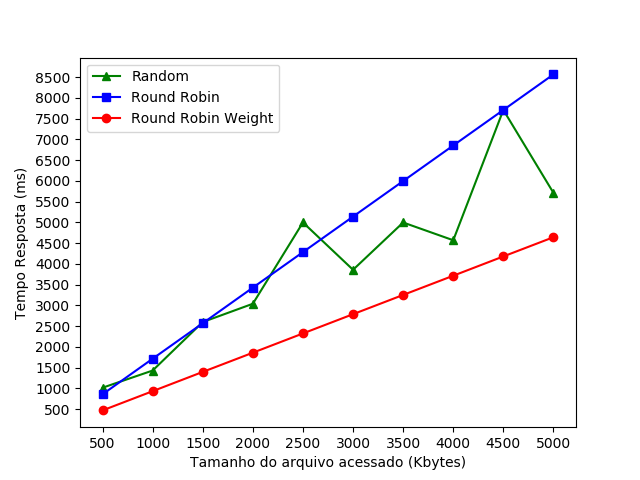
\includegraphics[width=\textwidth]{images/exp1_time.png}
            \caption{Relação entre o tamanho do arquivo e o tempo de acesso.}
            \label{fig:a}
        \end{minipage}
        \hspace{0.5cm}
        \begin{minipage}[b]{0.45\linewidth}
            \centering
            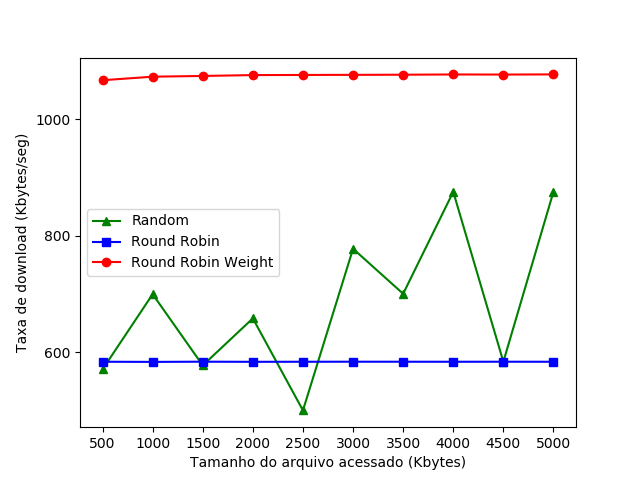
\includegraphics[width=\textwidth]{images/exp1_banda.png}
            \caption{Relação entre o tamanho do arquivo e a taxa de download.}
            \label{fig:b}
        \end{minipage}
    \end{figure}
\end{frame}  

\begin{frame}{Resultados obtidos - Experimento 2}

    Simula um cenário de homogeneidade de largura de banda disponível. O link entre todos os servidores e o \textit{Load Balancer} foram mantidos exatamente iguais, 10 MBits/s, 

    \begin{figure}[ht]
        \begin{minipage}[b]{0.45\linewidth}
            \centering
            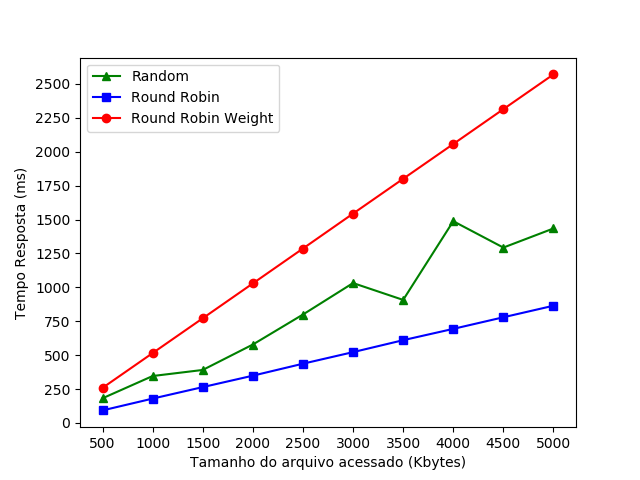
\includegraphics[width=\textwidth]{images/exp2_time.png}
            \caption{Relação entre o tamanho do arquivo e o tempo de acesso.}
            \label{fig:a}
        \end{minipage}
        \hspace{0.5cm}
        \begin{minipage}[b]{0.45\linewidth}
            \centering
            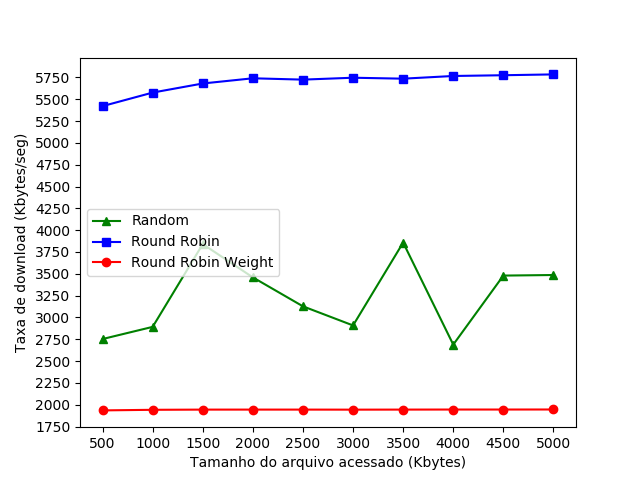
\includegraphics[width=\textwidth]{images/exp2_banda.png}
            \caption{Relação entre o tamanho do arquivo e a taxa de download.}
            \label{fig:b}
        \end{minipage}
    \end{figure}
\end{frame}  

\begin{frame}{Resultados obtidos - Experimento 3}

    Simula um cenário onde a metade dos servidores possuíam metade da banda dos outros servidores. 

    \begin{figure}[ht]
        \begin{minipage}[b]{0.45\linewidth}
            \centering
            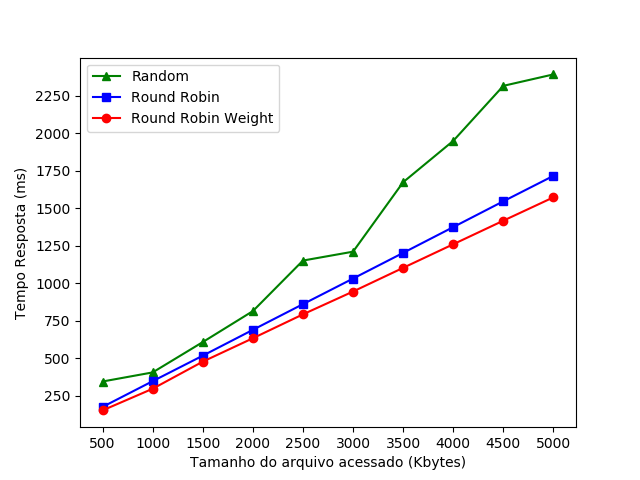
\includegraphics[width=\textwidth]{images/exp3_time.png}
            \caption{Relação entre o tamanho do arquivo e o tempo de acesso.}
            \label{fig:a}
        \end{minipage}
        \hspace{0.5cm}
        \begin{minipage}[b]{0.45\linewidth}
            \centering
            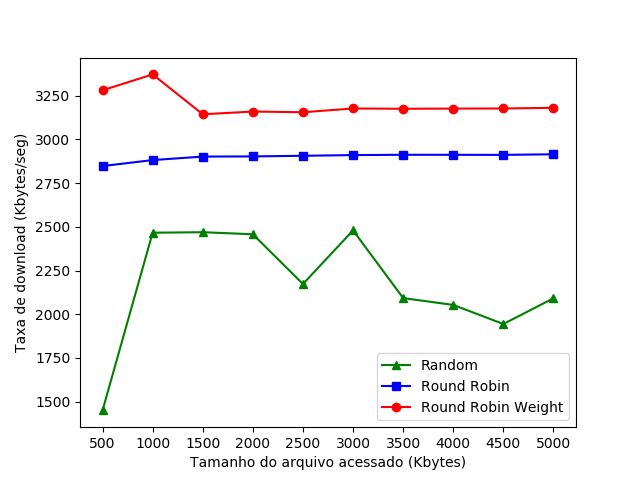
\includegraphics[width=\textwidth]{images/exp3_banda.png}
            \caption{Relação entre o tamanho do arquivo e a taxa de download.}
            \label{fig:b}
        \end{minipage}
    \end{figure}
\end{frame}  

\begin{frame}{Considerações finais}
    \begin{itemize}  
        \item  Usando o teste de hipótese não paramétrico \textit{Kruskal-Wallis} não podemos rejeitar a hipótese h0;
        \item Simulações realizadas utilizando o controlador Pox e o simulador Mininet;
        \item Os resultados desse experimento foram comparados com os obtidos por [Kaur, 2015] e os resultados que obtivemos não são similares aos resultados apresentados pelos autores no referido artigo.;
    \end{itemize}
    
\end{frame}  


\begin{frame}{Considerações finais}

\begin{table}[h]
\centering
\caption{Quando comparativo entre os diferentes cenários e os tipos de algorítimos utilizados}
\label{quadro_comparativo}
\begin{tabular}{lccc}
 & \multicolumn{1}{l}{\textbf{Random}} & \multicolumn{1}{l}{\textbf{Round Robin}} & \multicolumn{1}{l}{\textbf{RRW}} \\\hline
\textbf{Balanceado} &  & X &  \\
\textbf{Desbalanceado} &  &  & X \\
\textbf{Homogêneo} & X & X & 
\end{tabular}
\end{table}
    
\end{frame}  

\begin{frame}{Referências}
    kaur, S., Kumar, K., Singh, J., and Ghumman, N. S. (2015).   Round-robin based loadbalancing in software defined networking.  In2015 2nd International Conference onComputing for Sustainable Global Development (INDIACom), pages 2136–2139.

\end{frame}  


\end{document}
